%%%%%%%%%%%%%%%%%%%%%%%%%%%%%%%%%%%%%%%%%%%%%%%%%%%%%%%%%%%%%%%%%%%%%%%%%%%%
% AGUJournalTemplate.tex: this template file is for articles formatted with LaTeX
%
% This file includes commands and instructions
% given in the order necessary to produce a final output that will
% satisfy AGU requirements, including customized APA reference formatting.
%
% You may copy this file and give it your
% article name, and enter your text.
%
% guidelines and troubleshooting are here: 

%% To submit your paper:
\documentclass[draft]{agujournal2019}
\usepackage{url} %this package should fix any errors with URLs in refs.
\usepackage{lineno}
\usepackage[inline]{trackchanges} %for better track changes. finalnew option will compile document with changes incorporated.
\usepackage{soul}
\usepackage{wrapfig}
\linenumbers
%%%%%%%
% As of 2018 we recommend use of the TrackChanges package to mark revisions.
% The trackchanges package adds five new LaTeX commands:
%
%  \note[editor]{The note}
%  \annote[editor]{Text to annotate}{The note}
%  \add[editor]{Text to add}
%  \remove[editor]{Text to remove}
%  \change[editor]{Text to remove}{Text to add}
%
% complete documentation is here: http://trackchanges.sourceforge.net/
%%%%%%%

\draftfalse

%% Enter journal name below.
%% Choose from this list of Journals:
%
% JGR: Atmospheres
% JGR: Biogeosciences
% JGR: Earth Surface
% JGR: Oceans
% JGR: Planets
% JGR: Solid Earth
% JGR: Space Physics
% Global Biogeochemical Cycles
% Geophysical Research Letters
% Paleoceanography and Paleoclimatology
% Radio Science
% Reviews of Geophysics
% Tectonics
% Space Weather
% Water Resources Research
% Geochemistry, Geophysics, Geosystems
% Journal of Advances in Modeling Earth Systems (JAMES)
% Earth's Future
% Earth and Space Science
% Geohealth
%
% ie, \journalname{Water Resources Research}

\journalname{Enter journal name here}


\begin{document}

%%%%%%%%%%%%%%%%%%%%%%%%%%%%%%%%%%%%%%%%%%%%%%%
%  TITLE
%
% (A title should be specific, informative, and brief. Use
% abbreviations only if they are defined in the abstract. Titles that
% start with general keywords then specific terms are optimized in
% searches)
%
%%%%%%%%%%%%%%%%%%%%%%%%%%%%%%%%%%%%%%%%%%%%%%%

% Example: \title{This is a test title}

\title{=enter title here=}

%%%%%%%%%%%%%%%%%%%%%%%%%%%%%%%%%%%%%%%%%%%%%%%
%
%  AUTHORS AND AFFILIATIONS
%
%%%%%%%%%%%%%%%%%%%%%%%%%%%%%%%%%%%%%%%%%%%%%%%

% Authors are individuals who have significantly contributed to the
% research and preparation of the article. Group authors are allowed, if
% each author in the group is separately identified in an appendix.)

% List authors by first name or initial followed by last name and
% separated by commas. Use \affil{} to number affiliations, and
% \thanks{} for author notes.
% Additional author notes should be indicated with \thanks{} (for
% example, for current addresses).

% Example: \authors{A. B. Author\affil{1}\thanks{Current address, Antartica}, B. C. Author\affil{2,3}, and D. E.
% Author\affil{3,4}\thanks{Also funded by Monsanto.}}

\authors{=list all authors here=}


% \affiliation{1}{First Affiliation}
% \affiliation{2}{Second Affiliation}
% \affiliation{3}{Third Affiliation}
% \affiliation{4}{Fourth Affiliation}

\affiliation{=number=}{=Affiliation Address=}
%(repeat as many times as is necessary)


% Corresponding author mailing address and e-mail address:

% (include name and email addresses of the corresponding author.  More
% than one corresponding author is allowed in this LaTeX file and for
% publication; but only one corresponding author is allowed in our
% editorial system.)

% Example: \correspondingauthor{First and Last Name}{email@address.edu}

\correspondingauthor{=name=}{=email address=}



%%%%%%%%%%%%%%%%%%%%%%%%%%%%%%%%%%%%%%%%%%%%%%%
% KEY POINTS
%%%%%%%%%%%%%%%%%%%%%%%%%%%%%%%%%%%%%%%%%%%%%%%
%  List up to three key points (at least one is required)
%  Key Points summarize the main points and conclusions of the article
%  Each must be 140 characters or fewer with no special characters or punctuation and must be complete sentences

% Example:
% \begin{keypoints}
% \item	List up to three key points (at least one is required)
% \item	Key Points summarize the main points and conclusions of the article
% \item	Each must be 140 characters or fewer with no special characters or punctuation and must be complete sentences
% \end{keypoints}

\begin{keypoints}
\item enter point 1 here
\item enter point 2 here
\item enter point 3 here
\end{keypoints}

%%%%%%%%%%%%%%%%%%%%%%%%%%%%%%%%%%%%%%%%%%%%%%%
%
%  ABSTRACT and PLAIN LANGUAGE SUMMARY
%
% A good Abstract will begin with a short description of the problem
% being addressed, briefly describe the new data or analyses, then
% briefly states the main conclusion(s) and how they are supported and
% uncertainties.

% The Plain Language Summary should be written for a broad audience,
% including journalists and the science-interested public, that will not have 
% a background in your field.
%
% A Plain Language Summary is required in GRL, JGR: Planets, JGR: Biogeosciences,
% JGR: Oceans, G-Cubed, Reviews of Geophysics, and JAMES.
% see http://sharingscience.agu.org/creating-plain-language-summary/)
%
%%%%%%%%%%%%%%%%%%%%%%%%%%%%%%%%%%%%%%%%%%%%%%%

%% \begin{abstract} starts the second page

\begin{abstract}
[ enter your Abstract here ]
\end{abstract}

\section*{Plain Language Summary}
Enter your Plain Language Summary here or delete this section.
Here are instructions on writing a Plain Language Summary: 
https://www.agu.org/Share-and-Advocate/Share/Community/Plain-language-summary


%%%%%%%%%%%%%%%%%%%%%%%%%%%%%%%%%%%%%%%%%%%%%%%
%
%  BODY TEXT
%
%%%%%%%%%%%%%%%%%%%%%%%%%%%%%%%%%%%%%%%%%%%%%%%

%%% Suggested section heads:
% \section{Introduction}
%
% The main text should start with an introduction. Except for short
% manuscripts (such as comments and replies), the text should be divided
% into sections, each with its own heading.

% Headings should be sentence fragments and do not begin with a
% lowercase letter or number. Examples of good headings are:

% \section{Materials and Methods}
% Here is text on Materials and Methods.
%
% \subsection{A descriptive heading about methods}
% More about Methods.
%
% \section{Data} (Or section title might be a descriptive heading about data)
%
% \section{Results} (Or section title might be a descriptive heading about the
% results)
%
% \section{Conclusions}

\section{Introduction}\label{intro}
% examples of citation formatting: 
% \cite{Arthun2012}
% \citeA{Arthun2012}

% global context, why are we interested in the Arctic, Arctic Amplification; regional feedback mechanisms with sea ice loss, how does Arctic circulation, heat fluxes and water masses require use to understand transformation process
% FIGURE 1 to include: an Arctic map of Bathymetry or two of heat/freshwater content anomalies
% mean velocity of the Barents Sea AW layer to show the direction of flow
% start big, make this smaller and smaller until the Barents Sea
It is well-established that the Arctic is warming at a substantially faster rate than anywhere else on Earth in a process known as Arctic Amplification (AA) \cite{Manabe1980,Serreze2009,Cosimo2014,Huang2017,Rantanen2022}. This amplification results from several interrelated feedback mechanisms, though the relative contributions of each are still debated \cite{Pithan2014,Timmermans2018,Gong2017,Pistone2019,Previdi2021}. One important driver of AA is the rapid decline in winter sea ice extent and thickness \cite{Perovich2009,Dai2019}, closely linked to ocean heat transport and changes in surface heat forcing \cite{Onarheim2018,Stroeve2018,Oldenburg2024}. The implications of this amplification extend beyond the Arctic; warming in the lower troposphere over the Arctic can potentially influence mid-latitude weather patterns \cite{Honda2009,Petoukhov2010,Francis2012,Cohen2018,Coumou2018}. Along the inflow pathways from the Pacific and Atlantic, borealization—the process by which strengthened inflows of increasingly warm waters and sea ice retreat drive sub-Arctic regions to adopt features typical of southern boreal ecosystems—is altering species distributions and migratory patterns, with cascading effects on local economies and global biodiversity \cite{Fossheim2015,Polyakov2020_borealization,Ingvaldsen2021,Husson2024}. AA is not uniform, nor is the warming of the ocean explained by the changing atmosphere alone \cite{Marshall2014}. Winter sea ice decline and surface air temperature (SAT) amplification the highest globally in the Northern Barents sea, making it stand out as a focal point for Arctic change \cite{Screen2010,Onarheim2017,Isaksen2022,Rantanen2022}.

% what is happening in the Barents Sea and mechanisms causing this change
The Barents Sea has experienced a steady increase in heat content over recent decades \cite{Smedsrud2013,Bianco2024}, accompanied by a decline in near-surface freshwater content \cite{Watelet2020}. These changes are altering ocean stratification throughout the sea \cite{Lind2018,Hordoir2022}. A key mechanism behind these changes is the rapid sea ice reduction \cite{Rieke2023}, which can be attributed in part to the increased volume and warming of Atlantic inflow \cite{Smedsrud2010,Onarheim2018,Smedsrud2022}. This warm inflow and sea ice reduction reduces surface freshwater input, weakens stratification, and allows for enhanced vertical mixing, creating a feedback loop that accelerates "Atlantification," or the transformation of the Barents Sea into a warm, well-mixed Atlantic structure \cite{Arthun2012,Polyakov2017,Gerland2023}. During winter, when surface heat fluxes are negative, ocean heat transport (OHT) from the Atlantic inflow is the dominant cause of ice melt \cite{Ivanov2012,Tsubouchi2021}, increasing the ice-free area and amplifying surface heat release \cite{Skagseth2020}. The northward spread of warm, saline water \cite{Oziel2016} changes local ecologies \cite{Bogstad2015,Dalpadado2014,Ingvaldsen2021} and further erodes stratification \cite{Lind2018}. This warm water cools along its inflow path, but the ability of the Barents Sea to cool Atlantic inflow appears to be diminishing \cite{Shu2021,Skagseth2020}. These interlinked feedbacks--sea ice loss, atmospheric changes due to AA, and OHT--remain complex, and understanding their interactions is critical for predicting the future regimes of the region.

\begin{wrapfigure}{r}{0.65\textwidth}
    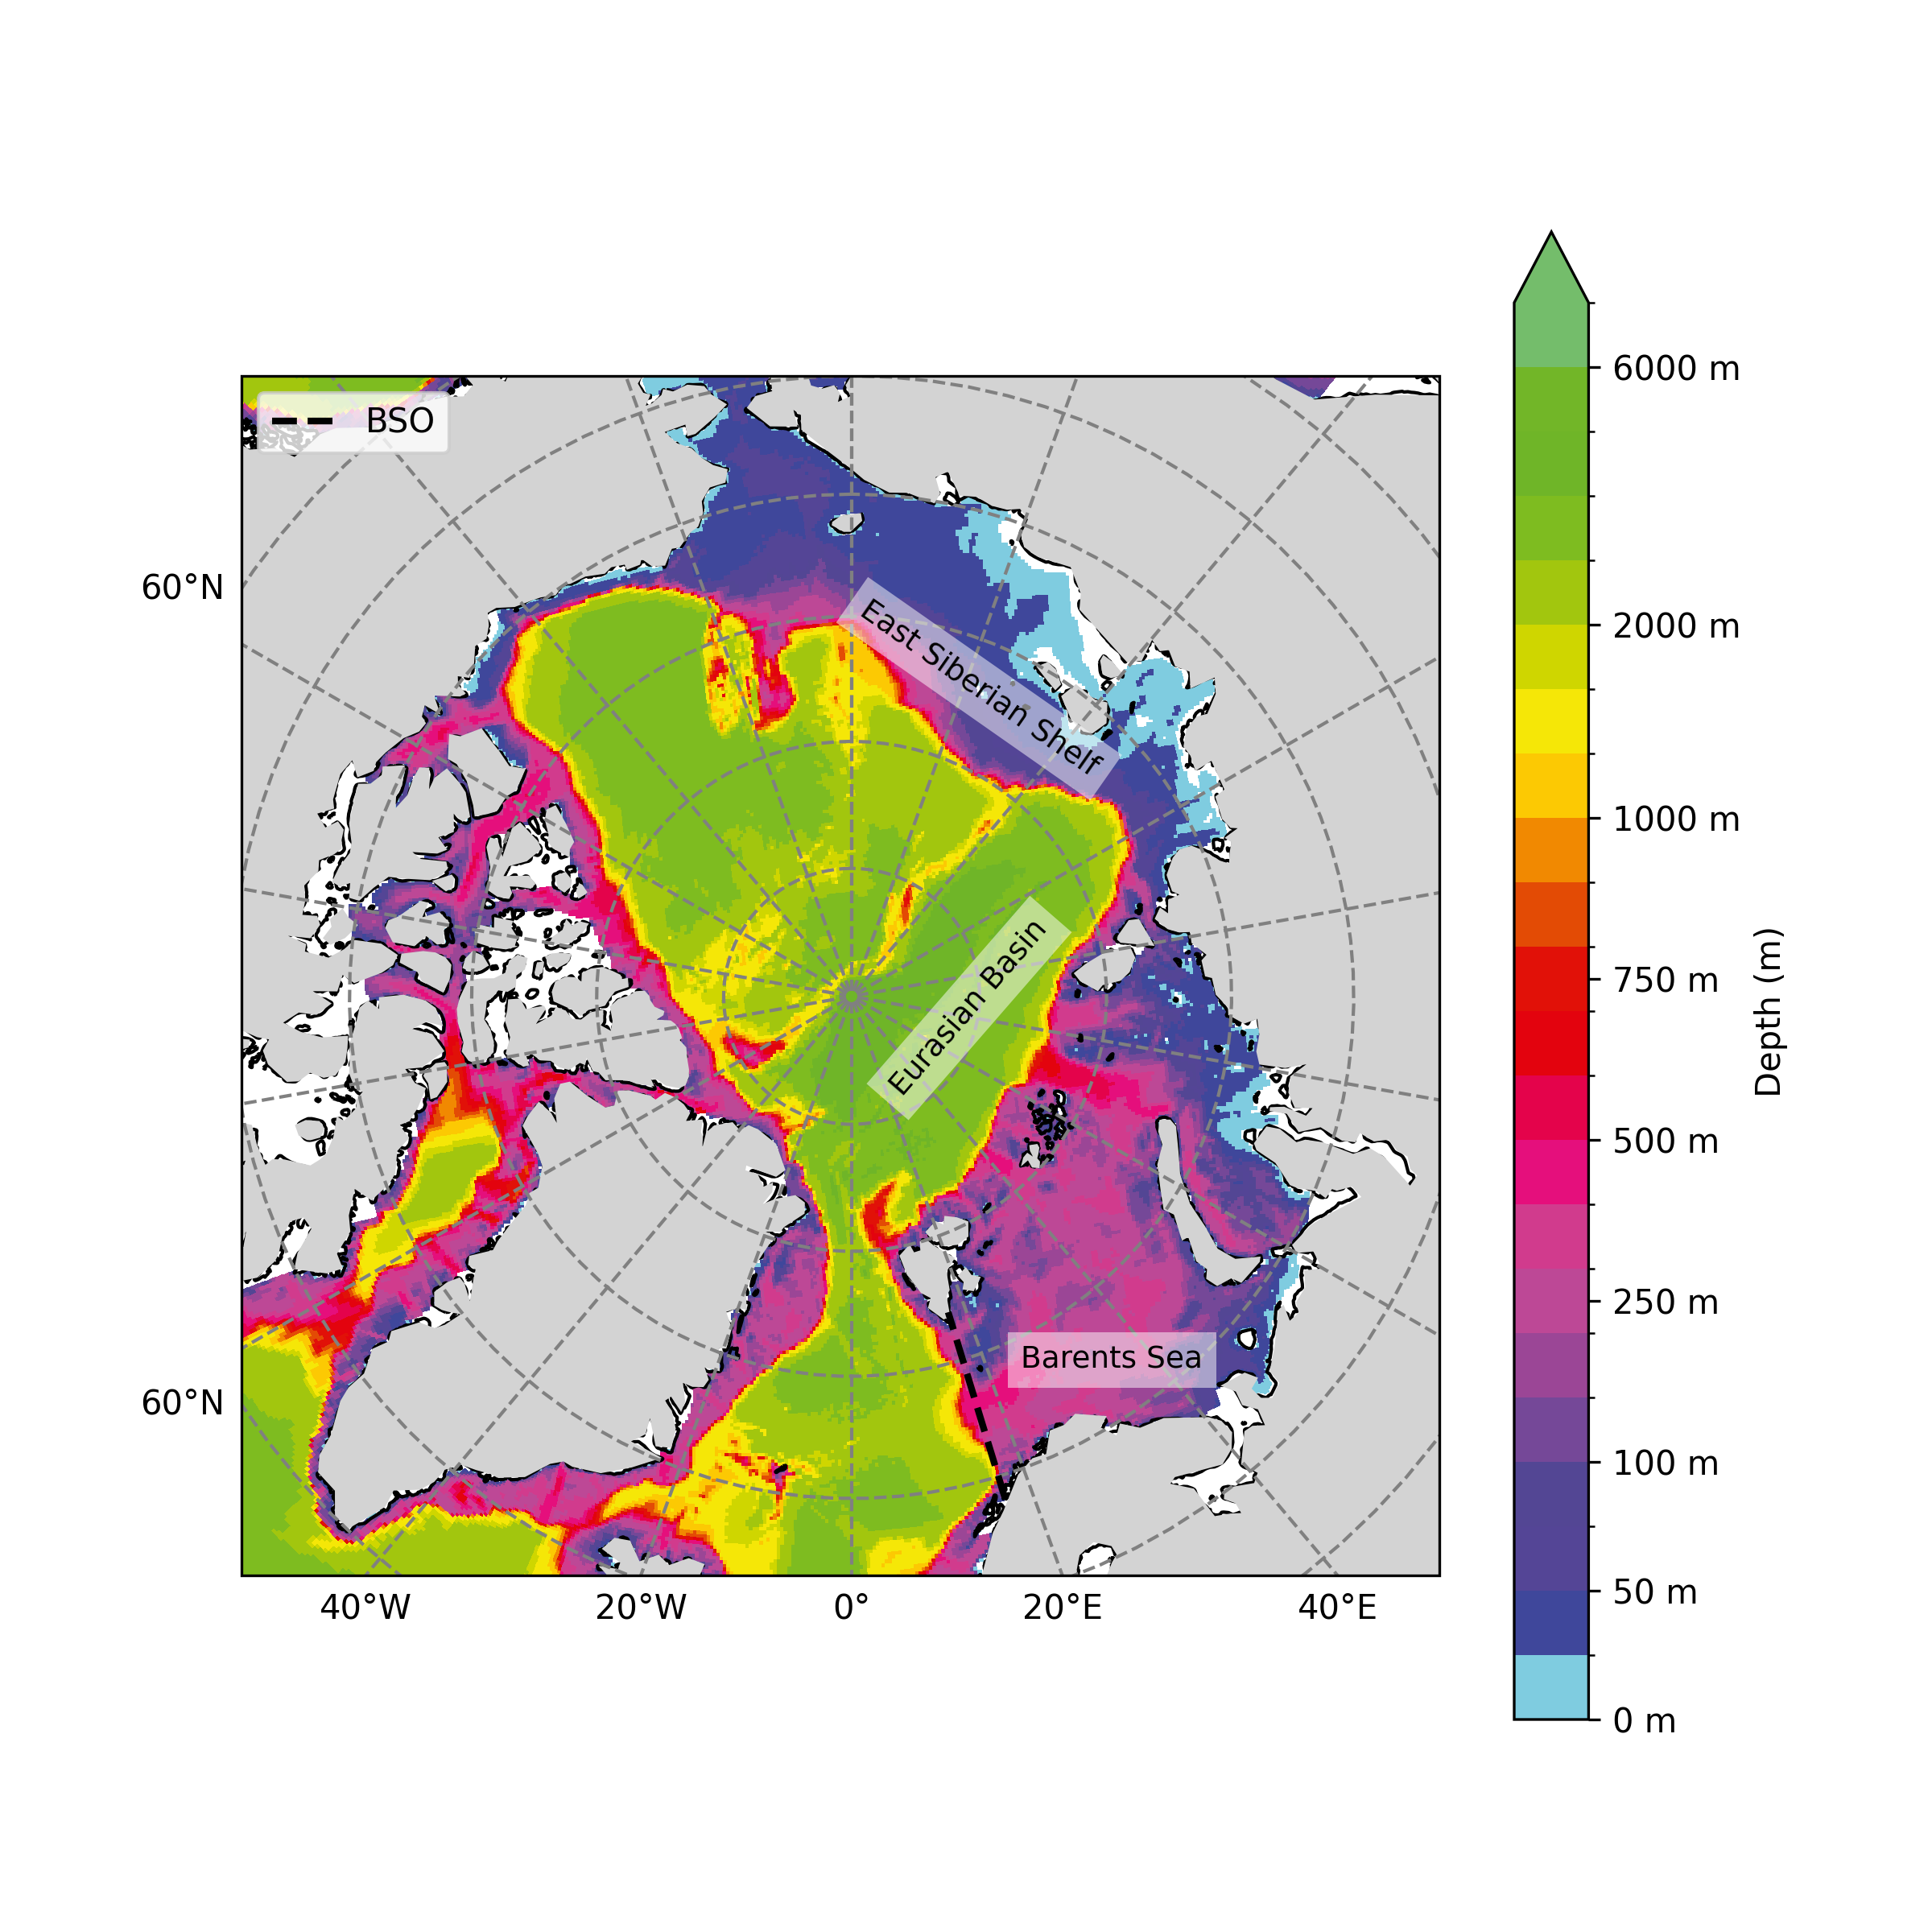
\includegraphics[width=\linewidth]{figs/ASTE_bathymetry_labels.png}
    \caption{Map of the Arctic Ocean.}
    \label{fig:timeseries}
\end{wrapfigure}

% barents sea structure and connection to the Arctic Ocean -- possibly remove info about the polar front and move it down next para
% . Thus, the processes influencing the strength and location of the PF, including sea ice extent, internal tides, and mesoscale dynamics, are critical factors in Atlantification .
The Barents Sea serves as a transition zone between the Arctic and Atlantic Oceans, and is shaped by two primary water masses, each defined by their temperature (\emph{T}) and salinity (\emph{S}): warm, saline Atlantic Water (AW) entering through the Barents Sea Opening (BSO) and cold, fresh Arctic Water (ArW) flowing southward from the Arctic Ocean \cite{Loeng1991,Smedsrud2010}. The boundary between these regimes is the Polar Front (PF), an oceanic feature marked by strong lateral gradients in temperature and salinity. In the western Barents Sea, the PF is steered by bathymetry, whereas in the East, the front broadens and splits into distinct temperature and salinity fronts \cite{Oziel2016}. The PF governs the geographic region where AW can lose heat to the atmosphere and freshen from sea ice melt, precipitation, and runoff before it is subducted beneath ArW and enters the Arctic Basin through the St. Anna Trough. These surface processes play a key role in preconditioning heat and salt transported to the central Arctic \cite{Parsons1996,Munk1998,Garrett2003,Vage2014,kolas2024}. Upon entering the Arctic Ocean, AW encounters another inflow branch from the Fram Strait. Together, these waters propagate along the continental slope as part of the Arctic Ocean Boundary Current system, which circulates clockwise around the Arctic Basin \cite{Wang2020}. This circulation redistributes heat and salt along the Eurasian and Canadian margins, playing a crucial role in modifying the Arctic halocline—a cold, salty layer that insulates sea ice from the warmer AW below. However, increasing heat content from Atlantification in the Barents Sea has intensified temperature gradients across the PF, limiting sea ice extent \cite{Barton18}, and weakening the cold halocline layer, particularly along the Eurasian shelf \cite{Polyakov2020,Metzner2020}. This has implications for the stability of the Arctic Ocean stratification and the vertical distribution of heat, which could exacerbate ice loss and alter circulation patterns across the basin. South of the PF, the Barents Sea is strongly influenced by AW inflow \cite{Hakkinen2009}. In contrast, the northern Barents Sea exhibits salinity-driven stratification, sustained by ice melt and resembling Arctic conditions \cite{kolas2024}. The salt-stratified northern regime is often referred to as a "beta" ocean \cite{Nansen1902,Carmack2007,Stewart2016}; contrasting this is the "alpha" ocean, which describes most of the global oceans and is primarily temperature-stratified. The interaction of AW and ArW within the stratified environment of the Barents Sea has implications for the Arctic Ocean circulation, as AW holds enough heat to melt Arctic sea ice were it hypothetically to reach the surface \cite{Polyakov2017,Stroeve2018,Grabon2021}. Understanding these dynamics is crucial for evaluating the broader impacts of Atlantification on the Arctic system.

% weakening cold halocline later : \cite{Polyakov2020,Metzner2020}.

% PF is typically defined by the Northern Front which is salinity (Oziel, Barton)

% \begin{wrapfigure}{r}{0.5\textwidth}
%     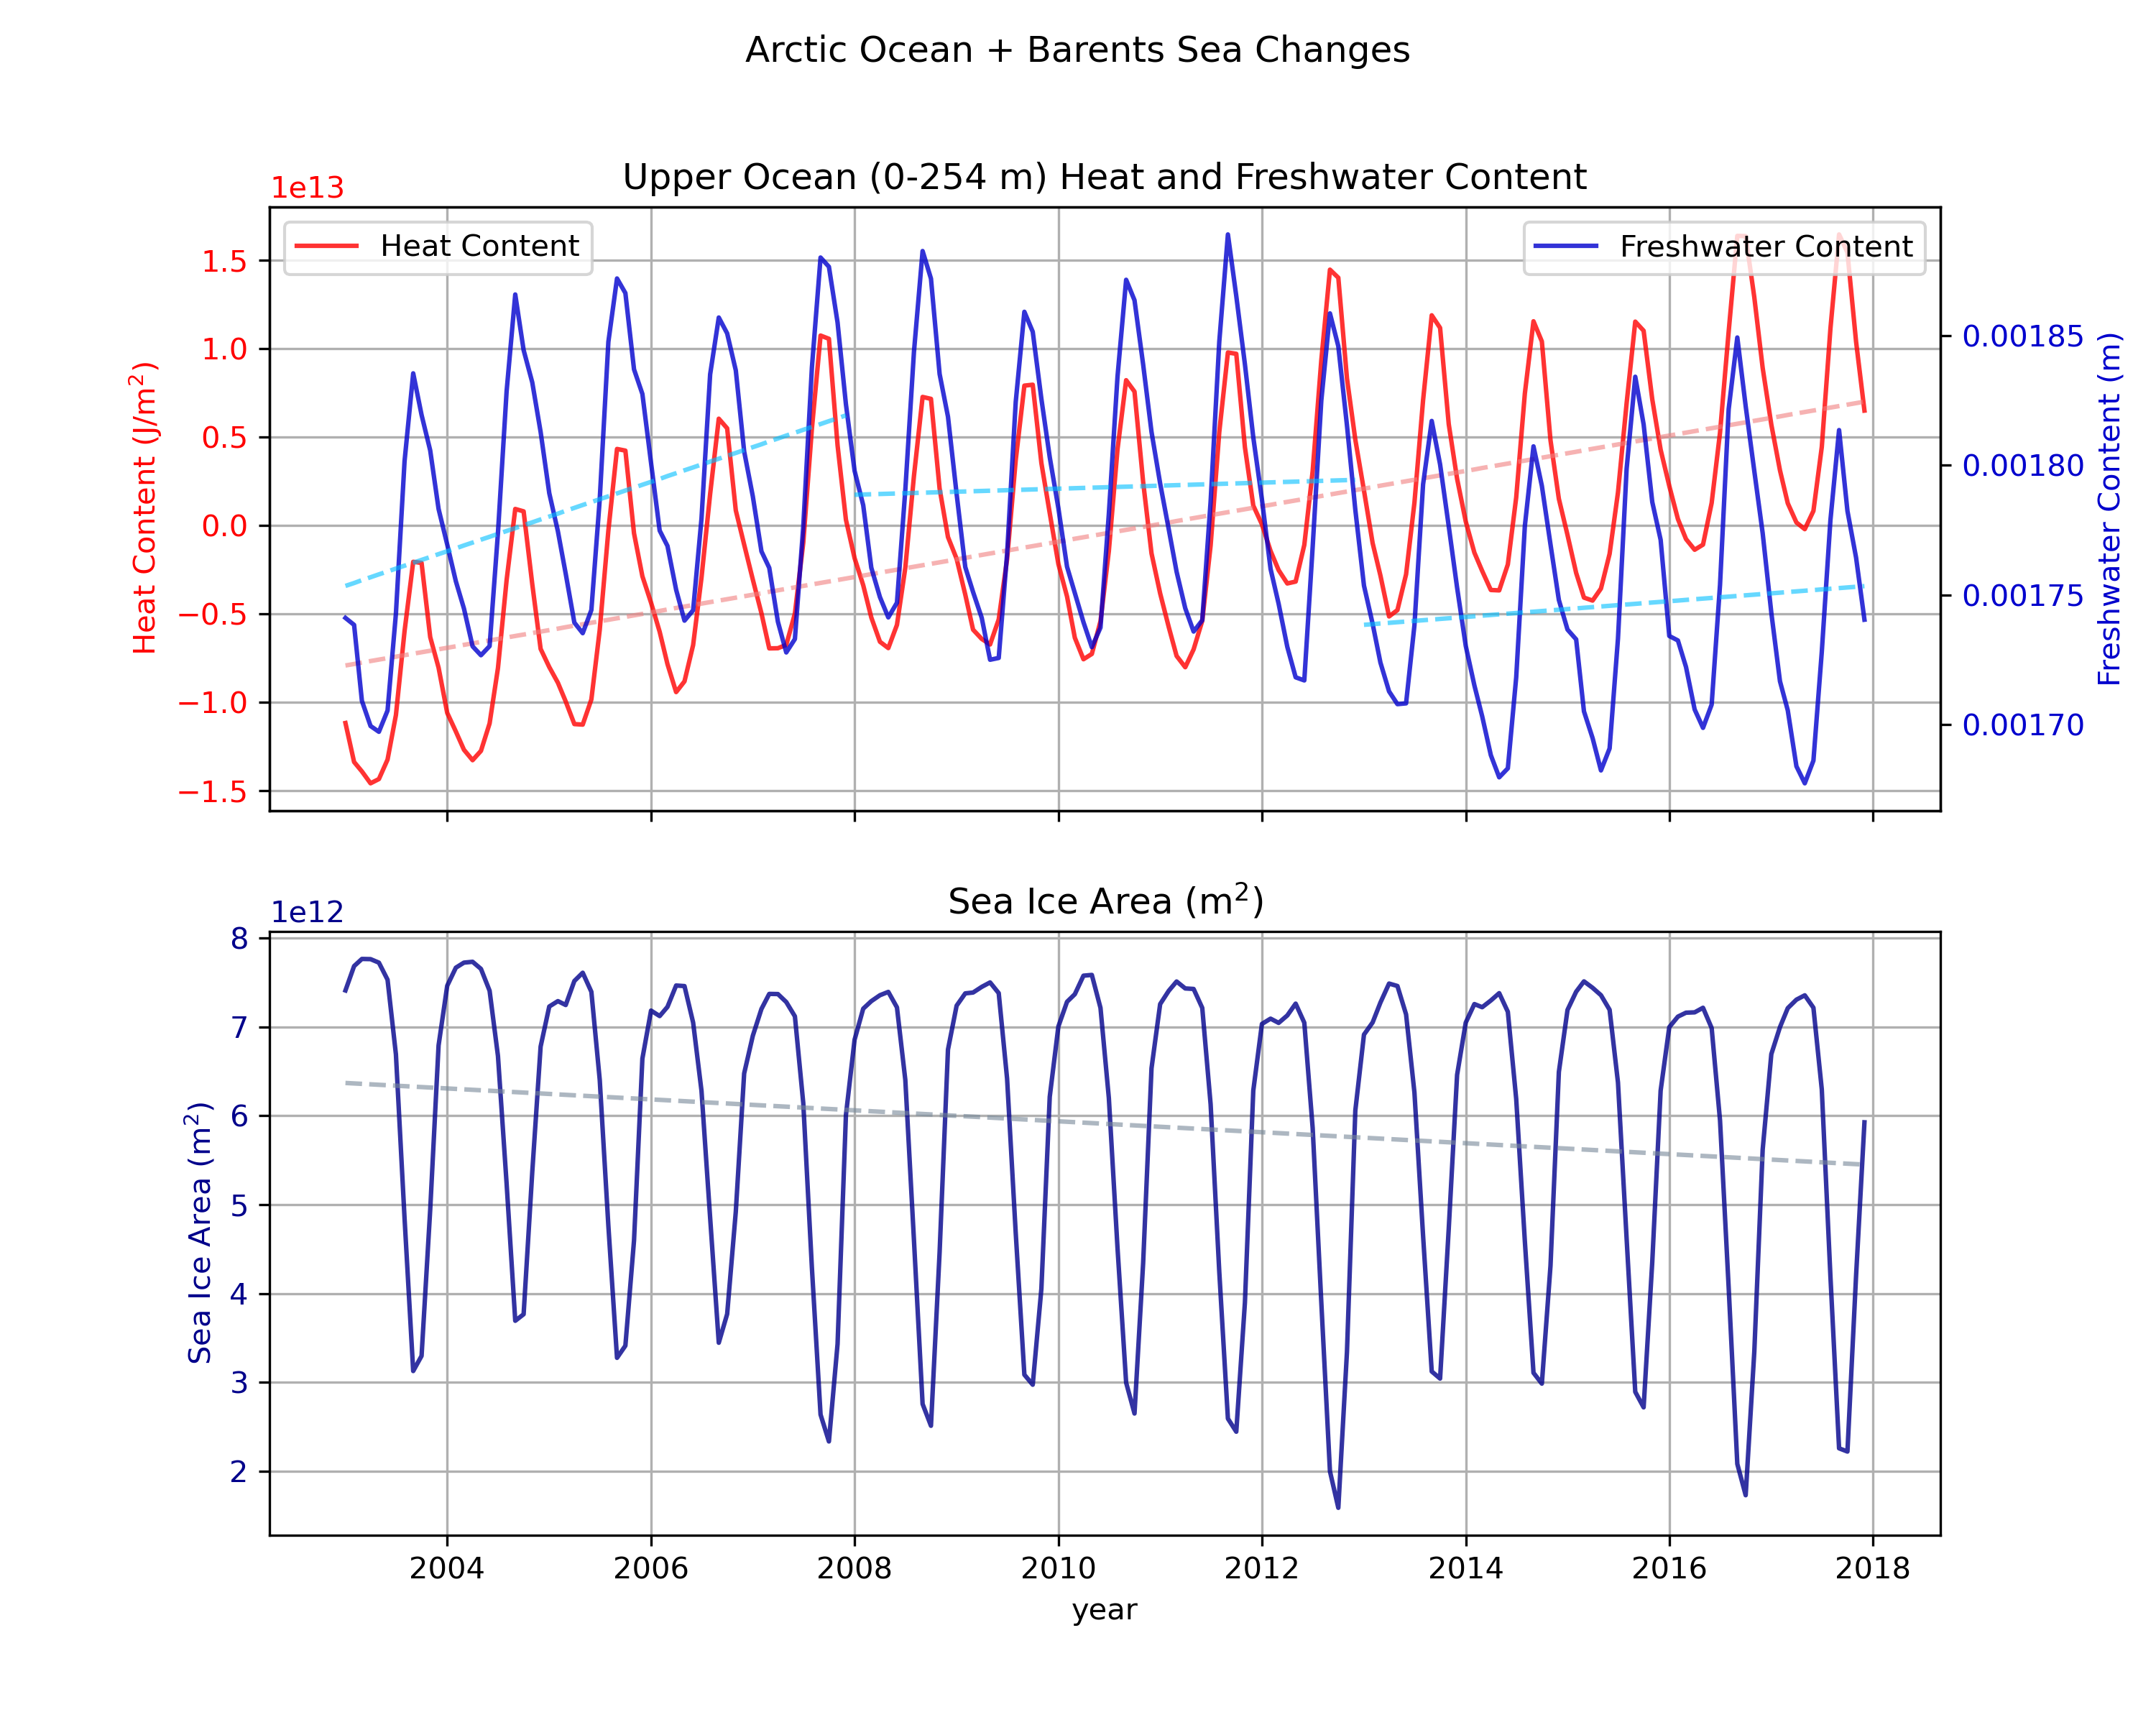
\includegraphics[width=\linewidth]{figs/Arctic_timeseries_proposal.png}
%     \caption{This is an example figure and caption that will be changed later...}
%     \label{fig:timeseries}
% \end{wrapfigure}

% fluid dynamics 
The large-scale dynamical impacts of Atlantification, sea ice retreat, and atmospheric heating can be considered through the laws of fluid dynamics to redistribute heat and salt in the ocean. Heat and salt in the ocean are directly tied to temperature (\emph{T}) and salinity (\emph{S}), with heat corresponding to the thermal energy that drives \emph{T} variations, and \emph{S} representing the concentration of dissolved salts. Together with pressure, which increases with depth, these properties influence the density of seawater, with colder, saltier water being denser than warmer, fresher water. Gravity plays a fundamental role in establishing and maintaining this density-driven stratification, as described by Archimedes' principle: a fluid parcel experiences an upward buoyant force proportional to the density difference with its surroundings, counteracting the downward pull of gravity. This balance creates a stable thermohaline stratification in the ocean in which denser layers are deeper than less dense ones, forming near-parallel isopycnal surfaces that extend across the ocean. Incorporating buoyancy, the vertical momentum equation can be expressed as:

$$
\frac{Dw}{Dt} = -\frac{1}{\rho_0} \frac{\partial p}{\partial z} + b
$$

where $\frac{Dw}{Dt}$ represents the vertical acceleration, ${\rho_0}$ is the reference density of the ocean (1029 $\frac{kg}{m^3}$), $\frac{\partial p}{\partial z}$ is the vertical pressure gradient, and $b$ is the buoyancy term, where $b = -g \frac{\rho'}{\rho_0}$. A positive buoyancy can lead to upward acceleration, and a negative buoyancy can lead to downward acceleration. In a stably stratified ocean, gravity acts to maintain this layered structure; mixing across these isopycnals requires an external energy input.


% how is this system disrupted
The stability of the ocean is are static and can be disrupted by surface fluxes of heat and freshwater \cite{Speer1993}, and heat and salt redistributed by advection and diffusion \cite{StoleHansen1991,long2017}. Large scale circulation, such as the northward flow of AW, exemplifies advection, transporting heat and salt along isopycnals into regions where these properties are otherwise scarce. This advection establishes strong density gradients, which are a prerequisite for baroclinic instability--a process that generates potential energy and drives mesoscale eddies. These eddies play a pivotal role in diffusing heat and salt along isopycnals, effectively homogenizing ocean properties and reducing the ranges of \emph{T} and \emph{S}. In addition to isopycnal diffusion by eddies, molecular diffusion acts diapycnally, transferring heat and salt across isopycnals from warmer to cooler and saltier to fresher regions, yet these effects are small compared to the larger-scale processes associated with mesoscale eddies. Together, advection and diffusion form a coupled mechanism to redistribute heat and salt across the ocean, altering thermohaline stratification, as described by \citeA{Munk1966}. In the Barents Sea, the relative roles of these processes are shifting due to climate change. As the composition of inflowing AW shifts, so too are the gradients in \emph{T} and \emph{S}, enhancing potential vorticity (PV) gradients and limiting the expansion of sea ice across the PF \cite{Oziel2016,Barton18}. Increased wind stress over an increasingly ice-free ocean amplifies this eddy activity \cite{Shao2023,li2024eddy}, enhancing the redistribution of ocean properties at the PF \cite{Porter2020}. However, at the PF, mesoscale eddies enable some degree of cross-frontal exchange and have been noted as a potential cause of weakened stratification of the sea \cite{kolas2024}. Furthermore, the shortening of the freezing period increases the influence of atmospheric forcing on surface heating \cite{Dorr2024}, further underscoring the relevance of the changes occurring in this region. 


% Cole 2015, 
% intro paragraph on WMT -- what it is and why do we care
% summarizee some insights provided by earlier studies on why the WMT framework is useful
One approach to quantify the changes in \emph{T} and \emph{S} is through the water mass transformation (WMT) framework. Water masses, defined by discrete sets of \emph{T} and \emph{S} coordinates, have long been used to study the layering and large scale circulation in the ocean because of their relation to ocean density \cite{sverdrup1942}. In this framework, a "transformation" describes the process by which one ocean water mass--defined as a discrete volume of water--is converted into another through changes in \emph{T} and \emph{S} driven by mechanisms such as advection, internal diffusion, and surface fluxes. Because seawater density and stratification depend directly on these variables, understanding their distribution offers  valuable information on the circulation of the ocean.

% state of the art/history of literatutre
Substantial effort has been undertaken to develop a WMT framework for the ocean in tracer coordinates. In the first paper of its kind, \citeA{Walin_1977} described ocean salinity changes as flux- and mixing-driven volume transport across isohaline surfaces. In a subsequent paper, \citeA{Walin1982} showed that volume flow across isothermal surfaces can be used to study the impact of advective and diffusive heat fluxes at the ocean surface on the temperature distribution of the ocean. These two papers thus laid the foundation for descriptions of WMT in tracer--not geographic--coordinates, enabling water mass formation calculations from air-sea fluxes. \citeA{Speer1993} generalized the \citeA{Walin_1977, Walin1982} framework to use \emph{S} and \emph{T} coordinates simultaneously, using the continuity equations to show how the thermodynamic budgets for heat and freshwater can be used to describe WMT due to heat and freshwater fluxes. His work used a two-dimensional vector to describe the conversion rate of one water mass into another. This rate describes the volume flux across isothermal or isohaline surfaces, with the volume of water between these layers as a water mass. At the edges of these thermohaline surfaces, surface forcing can add or remove salt or heat, thus pushing the boundary outward or inward, while internal diffusion can smooth gradients at the boundary, causing mixing that can shift the edges. Advection, by the conservation of mass, cannot alter the total volume of a thermohaline layer but can deform or displace these surfaces. For instance, advection may shift the location of these surfaces horizontally or vertically, strengthening or weakening stratification. Furthermore, advection can change the near-surface \emph{T} and \emph{S} gradients, thus modifying the local exchange of heat and freshwater with the atmosphere or facilitating mixing. The transformation rates introduced by \citeA{Walin1982} quantify the shifts across these thermohaline surfaces as transformation rates; it is the divergence of these rates that indicate the net rate at which a water mass is formed or destroyed. This means that advection contributes indirectly by redistributing water properties, altering fluxes across the surface and influencing the accumulation or destruction of certain water masses. To synthesize these ideas into a broader framework, \citeA{doos2012} and \citeA{zika2012} introduced the thermohaline streamfunction, intended to show that in a steady state, transformation vectors for the global ocean show no net-convergence; this streamfunction was in fact nonzero. \citeA{Groeskamp2014} further developed the streamfunction to account for the instantaneous velocity and the movement of isohaline and isothermal surfaces in time. 

% establishing the use of \emph{T}--\emph{S} analysis as an approach to studying WMT and making it possible to calculate the convergence of any given water mass due to surface processes.

% the T--S framework
\emph{T}--\emph{S} analysis, formalized by \citeA{Hieronymus2014}, provides a powerful framework for understanding WMT. Developed from \citeA{Walin1982}, the \citeA{Hieronymus2014} framework formulated a continuity equation in \emph{T}--\emph{S} space, enabling the decomposition of WMT drivers into process-specific terms using a transformation vector. Building on the setup of \citeA{Speer1993}, \citeA{Hieronymus2014} incorporated isoneutral and dianeutral mixing, allowing for a breakdown of the influences on \emph{T} or \emph{S} independently. This breakdown of forcing terms was inspired from other studies which worked to quantify these processes using density alone \cite{Tziperman1986,Nurser1999,Marshall1999,Iudicone2008}, but the use of both \emph{T} or \emph{S} coordinates allows for a more nuanced representation of WMT. In this approach, traditional geographic coordinates (latitude, longitude, and depth) are translated into a two-dimensional \emph{T}--\emph{S} representation, allowing volumes of water within specific \emph{T} and \emph{S} ranges to be visualized. This framework is particularly effective for identifying water masses, analyzing their interactions, and studying mixing and circulation patterns on a process-based scale, rather than focusing solely on regional or basin-specific processes. \emph{T}--\emph{S} analysis is particularly beneficial in beta oceans, where analysis in \emph{T} or density alone would fail to account for surface freshwater influences on WMT. In the Arctic, \emph{T}--\emph{S} analysis helps to resolve both the impact of increased surface warming from AA and changes to freshwater forcing, providing a more comprehensive understanding of WMT and density changes. \citeA{Pemberton2015} applied the \citeA{Hieronymus2014} framework in the Arctic Ocean to investigate long-term mean transformations to study the interactions between Atlantic and Pacific inflows as well as ice dynamics.


% budget analysis
% \cite{Hieronymus2014}: This further allowed for the attribution of WMT to specific processes, but did not include convection or bottom boundary terms, and thus did not close a budget. 

% \cite{Pemberton2015}: While this application provided valuable insights into dominant, long-term transformation trends, it did not close the budget nor address shorter-term processes, leaving gaps in understanding the relative impacts of various transformation mechanisms in Arctic WMT.

% \cite{Evans2023}: wmt with residuals


% % paragraph introducing/motivating WMT in the Barents Sea/how has this been applied in other studies
% As the heat and salinity of the Barents Sea change, so too does its buoyancy. Ocean stratification is determined by buoyancy---a crucial term in the vertical momentum equation. Positive buoyancy drives upward acceleration, while negative buoyancy causes downward motion, influencing the stability of the water column. In a stratified ocean, buoyancy depends on density, which acts to restore displaced fluid particles to maintain equilibrium. In seawater, fluid density ($\rho$) depends on temperature and salt, but salinity changes exert a far greater impact on $\rho$. This makes salinity an important factor shaping stratification, particularly in polar regions where surface salt fluxes are substantial.


% WMT in the Barents Sea -- what's the point
% We employ a fully-closed WMT framework in \emph{T}--\emph{S} space for the Barents Sea. Closed budgets, derived from continuity equations, are essential for accurately capturing heat and freshwater variability by accounting for all contributing terms. The elimination of residuals thus allows us to ascertain the attribution of both dominant and minor physical processes on \emph{T} and \emph{S} changes. In the context of Atlantification in the Barents Sea, this framework is particularly valuable as it connects the changes in \emph{T} and \emph{S} to variations in density. The advection of AW is expected to play an important role in the observed warming and salinification of the Barents Sea, particularly in the northern, salinity-stratified regime. Surface heat fluxes and sea ice retreat further modulate surface transformation, reinforcing changes in the water column. Internal mixing contributes to WMT, homogenizing the previous contributions from advection and surface processes. Ultimately, the closed-budget WMT framework provides a comprehensive and nuanced understanding of the processes driving regime shifts in the Barents Sea, shedding light on the interplay between these processes.


% motivation and research questions; key gaps in knowledge; goals of the paper as quantifying WMT, identifying key drivers, and understanding their implications on the Arctic system
% (DRAFT) We hypothesize that the relative roles of AW import and surface process changes can be quantified using a budgeted WMT framework.


\section{Methodology}\label{methods}

\subsection{Model Description}

Here talk about ASTE

\subsection{WMT in a \emph{T}--\emph{S} Framework}

Here we will describe the basic equations of the T--S framework, including basic budgeting equations

% why is our budget analysis unique

% what is budget analysis

% INCLUDE the equations for this

% FIGURE 3: demonstrate budget analysis in T--S space

% FIGURE 4: for the 5 years; motivate this with figure 1 (SI extent timeseries)
% goal of this is to show that the advective term is changing over time as a contribution to heating and salting

\section{Results}

% FIGURE 5: highlight the convergence anomalies for the five years; compare this to figure 2 with the vertical stratification (redistribution away from the center to make a more average looking profile)
% focus on the one month (march) or maybe take a winter average motivated by the literature, use this for 2012 and 2014 to show that less sea ice -- less stratification -- redistribution of water away from the mixing line


%%

%  Numbered lines in equations:
%  To add line numbers to lines in equations,
%  \begin{linenomath*}
%  \begin{equation}
%  \end{equation}
%  \end{linenomath*}



%% Enter Figures and Tables near as possible to where they are first mentioned:
%
% DO NOT USE \psfrag or \subfigure commands.
%
% Figure captions go below the figure.
% Acronyms used in figure captions will be spelled out in the final, published version.

% Table titles go above tables;  other caption information
%  should be placed in last line of the table, using
% \multicolumn2l{$^a$ This is a table note.}
% NOTE that there is no difference between table caption and table heading in the final, published version
%
%----------------
% EXAMPLE FIGURES
%
% \begin{figure}
% \includegraphics{example.png}
% \caption{caption}
% \end{figure}
%
% Giving latex a width will help it to scale the figure properly. A simple trick is to use \textwidth. Try this if large figures run off the side of the page.
% \begin{figure}
% \noindent\includegraphics[width=\textwidth]{anothersample.png}
%\caption{caption}
%\label{pngfiguresample}
%\end{figure}
%
%
% If you get an error about an unknown bounding box, try specifying the width and height of the figure with the natwidth and natheight options. This is common when trying to add a PDF figure without pdflatex.
% \begin{figure}
% \noindent\includegraphics[natwidth=800px,natheight=600px]{samplefigure.pdf}
%\caption{caption}
%\label{pdffiguresample}
%\end{figure}
%
%
% PDFLatex does not seem to be able to process EPS figures. You may want to try the epstopdf package.
%

%
% ---------------
% EXAMPLE TABLE
%
% \begin{table}
% \caption{Time of the Transition Between Phase 1 and Phase 2$^{a}$}
% \centering
% \begin{tabular}{l c}
% \hline
%  Run  & Time (min)  \\
% \hline
%   $l1$  & 260   \\
%   $l2$  & 300   \\
%   $l3$  & 340   \\
%   $h1$  & 270   \\
%   $h2$  & 250   \\
%   $h3$  & 380   \\
%   $r1$  & 370   \\
%   $r2$  & 390   \\
% \hline
% \multicolumn{2}{l}{$^{a}$Footnote text here.}
% \end{tabular}
% \end{table}

%%%%%%%%%%%%%%%%%%%%%%%%%%%%%%%%%%%%%%%%%%%%%%%
% SIDEWAYS FIGURES and TABLES
% AGU prefers the use of {sidewaystable} over {landscapetable} as it causes fewer problems.
%
% \begin{sidewaysfigure}
% \includegraphics[width=20pc]{figsamp}
% \caption{caption here}
% \label{newfig}
% \end{sidewaysfigure}
%
%  \begin{sidewaystable}
%  \caption{Caption here}
% \label{tab:signif_gap_clos}
%  \begin{tabular}{ccc}
% one&two&three\\
% four&five&six
%  \end{tabular}
%  \end{sidewaystable}

%% If using numbered lines, please surround equations with \begin{linenomath*}...\end{linenomath*}
%\begin{linenomath*}
%\begin{equation}
%y|{f} \sim g(m, \sigma),
%\end{equation}
%\end{linenomath*}

%%% End of body of article

%%%%%%%%%%%%%%%%%%%%%%%%%%%%%%%%%%%%%%%%%%%%%%%
%% Optional Appendices go here
%
% The \appendix command resets counters and redefines section heads
%
% After typing \appendix
%
%\section{Here Is Appendix Title}
% will show
% A: Here Is Appendix Title
%
%\appendix
%\section{Here is a sample appendix}

%%%%%%%%%%%%%%%%%%%%%%%%%%%%%%%%%%%%%%%%%%%%%%%
% Optional Glossary, Notation or Acronym section goes here:
%
% Glossary is only allowed in Reviews of Geophysics
%  \begin{glossary}
%  \term{Term}
%   Term Definition here
%  \term{Term}
%   Term Definition here
%  \term{Term}
%   Term Definition here
%  \end{glossary}


%%%%%%%%%%%%%%%%%%%%%%%%%%%%%%%%%%%%%%%%%%%%%%%
% Acronyms
%% NOTE that acronyms in the final published version will be spelled out when used in figure captions.
%   \begin{acronyms}
%   \acro{Acronym}
%   Definition here
%   \acro{EMOS}
%   Ensemble model output statistics
%   \acro{ECMWF}
%   Centre for Medium-Range Weather Forecasts
%   \end{acronyms}


%%%%%%%%%%%%%%%%%%%%%%%%%%%%%%%%%%%%%%%%%%%%%%%
% Notation
%   \begin{notation}
%   \notation{$a+b$} Notation Definition here
%   \notation{$e=mc^2$}
%   Equation in German-born physicist Albert Einstein's theory of special
%  relativity that showed that the increased relativistic mass ($m$) of a
%  body comes from the energy of motion of the body—that is, its kinetic
%  energy ($E$)—divided by the speed of light squared ($c^2$).
%   \end{notation}




%%%%%%%%%%%%%%%%%%%%%%%%%%%%%%%%%%%%%%%%%%%%%%%
%
% DATA SECTION and ACKNOWLEDGMENTS
%
%%%%%%%%%%%%%%%%%%%%%%%%%%%%%%%%%%%%%%%%%%%%%%%

\section*{Open Research Section}
The ASTE\_R1 model configuration, inputs, and monthly and daily outputs are available at the Arctic Data Center (https://arcticdata.io).


\acknowledgments
Enter acknowledgments here. This section is to acknowledge funding, thank colleagues, enter any secondary affiliations, and so on.


%%%%%%%%%%%%%%%%%%%%%%%%%%%%%%%%%%%%%%%%%%%%%%%
% REFERENCES and BIBLIOGRAPHY
%
\bibliography{agusample} %don't specify the file extension
% don't specify bibliographystyle
%
%%%%%%%%%%%%%%%%%%%%%%%%%%%%%%%%%%%%%%%%%%%%%%%

%\bibliography{ enter your bibtex bibliography filename here }



%Reference citation instructions and examples:
%
% Please use ONLY \cite and \citeA for reference citations.
% \cite for parenthetical references
% ...as shown in recent studies (Simpson et al., 2019)
% \citeA for in-text citations
% ...Simpson et al. (2019) have shown...
%
%
%...as shown by \citeA{jskilby}.
%...as shown by \citeA{lewin76}, \citeA{carson86}, \citeA{bartoldy02}, and \citeA{rinaldi03}.
%...has been shown \cite{jskilbye}.
%...has been shown \cite{lewin76,carson86,bartoldy02,rinaldi03}.
%... \cite <i.e.>[]{lewin76,carson86,bartoldy02,rinaldi03}.
%...has been shown by \cite <e.g.,>[and others]{lewin76}.
%
% apacite uses < > for prenotes and [ ] for postnotes
% DO NOT use other cite commands (e.g., \citet, \citep, \citeyear, \nocite, \citealp, etc.).
%



\end{document}



More Information and Advice:

%%%%%%%%%%%%%%%%%%%%%%%%%%%%%%%%%%%%%%%%%%%%%%%
%
%  SECTION HEADS
%
%%%%%%%%%%%%%%%%%%%%%%%%%%%%%%%%%%%%%%%%%%%%%%%

% Capitalize the first letter of each word (except for
% prepositions, conjunctions, and articles that are
% three or fewer letters).

% AGU follows standard outline style; therefore, there cannot be a section 1 without
% a section 2, or a section 2.3.1 without a section 2.3.2.
% Please make sure your section numbers are balanced.
% ---------------
% Level 1 head
%
% Use the \section{} command to identify level 1 heads;
% type the appropriate head wording between the curly
% brackets, as shown below.
%
%An example:
%\section{Level 1 Head: Introduction}
%
% ---------------
% Level 2 head
%
% Use the \subsection{} command to identify level 2 heads.
%An example:
%\subsection{Level 2 Head}
%
% ---------------
% Level 3 head
%
% Use the \subsubsection{} command to identify level 3 heads
%An example:
%\subsubsection{Level 3 Head}
%
%---------------
% Level 4 head
%
% Use the \subsubsubsection{} command to identify level 3 heads
% An example:
%\subsubsubsection{Level 4 Head} An example.
%
%%%%%%%%%%%%%%%%%%%%%%%%%%%%%%%%%%%%%%%%%%%%%%%
%
%  IN-TEXT LISTS
%
%%%%%%%%%%%%%%%%%%%%%%%%%%%%%%%%%%%%%%%%%%%%%%%
%
% Do not use bulleted lists; enumerated lists are okay.
% \begin{enumerate}
% \item
% \item
% \item
% \end{enumerate}
%
%%%%%%%%%%%%%%%%%%%%%%%%%%%%%%%%%%%%%%%%%%%%%%%
%
%  EQUATIONS
%
%%%%%%%%%%%%%%%%%%%%%%%%%%%%%%%%%%%%%%%%%%%%%%%

% Single-line equations are centered.
% Equation arrays will appear left-aligned.

Math coded inside display math mode \[ ...\]
 will not be numbered, e.g.,:
 \[ x^2=y^2 + z^2\]

 Math coded inside \begin{equation} and \end{equation} will
 be automatically numbered, e.g.,:
 \begin{equation}
 x^2=y^2 + z^2
 \end{equation}


% To create multiline equations, use the
% \begin{eqnarray} and \end{eqnarray} environment
% as demonstrated below.
\begin{eqnarray}
  x_{1} & = & (x - x_{0}) \cos \Theta \nonumber \\
        && + (y - y_{0}) \sin \Theta  \nonumber \\
  y_{1} & = & -(x - x_{0}) \sin \Theta \nonumber \\
        && + (y - y_{0}) \cos \Theta.
\end{eqnarray}

%If you don't want an equation number, use the star form:
%\begin{eqnarray*}...\end{eqnarray*}

% Break each line at a sign of operation
% (+, -, etc.) if possible, with the sign of operation
% on the new line.

% Indent second and subsequent lines to align with
% the first character following the equal sign on the
% first line.

% Use an \hspace{} command to insert horizontal space
% into your equation if necessary. Place an appropriate
% unit of measure between the curly braces, e.g.
% \hspace{1in}; you may have to experiment to achieve
% the correct amount of space.


%%%%%%%%%%%%%%%%%%%%%%%%%%%%%%%%%%%%%%%%%%%%%%%
%
%  EQUATION NUMBERING: COUNTER
%
%%%%%%%%%%%%%%%%%%%%%%%%%%%%%%%%%%%%%%%%%%%%%%%

% You may change equation numbering by resetting
% the equation counter or by explicitly numbering
% an equation.

% To explicitly number an equation, type \eqnum{}
% (with the desired number between the brackets)
% after the \begin{equation} or \begin{eqnarray}
% command.  The \eqnum{} command will affect only
% the equation it appears with; LaTeX will number
% any equations appearing later in the manuscript
% according to the equation counter.
%

% If you have a multiline equation that needs only
% one equation number, use a \nonumber command in
% front of the double backslashes (\\) as shown in
% the multiline equation above.

% If you are using line numbers, remember to surround
% equations with \begin{linenomath*}...\end{linenomath*}

%  To add line numbers to lines in equations:
%  \begin{linenomath*}
%  \begin{equation}
%  \end{equation}
%  \end{linenomath*}



